\chapter{Introducción específica} % Main chapter title
\label{Chapter2}
%----------------------------------------------------------------------------------------
%	SECTION 1
%----------------------------------------------------------------------------------------
En este capítulo se presentan los requerimientos acordados con el cliente y los recursos de hardware (HW) y \textit{software} (SW) utilizados para el desarrollo del trabajo. Se describen en las partes implementadas del HW, los servicios integrados de \textit{backend} (BES) y solamente algunos aspectos relevantes del firmware (FW) que interactúa con el HW.\\
\section{Diagrama de bloques general del sistema}
El diagrama de bloques del HW a instalar \textit{in situ} es presentado en la figura \ref{fig:diagramadebloquesdelhw} y consta de cuatro bloques:
\begin{figure}[h!]
	\centering
	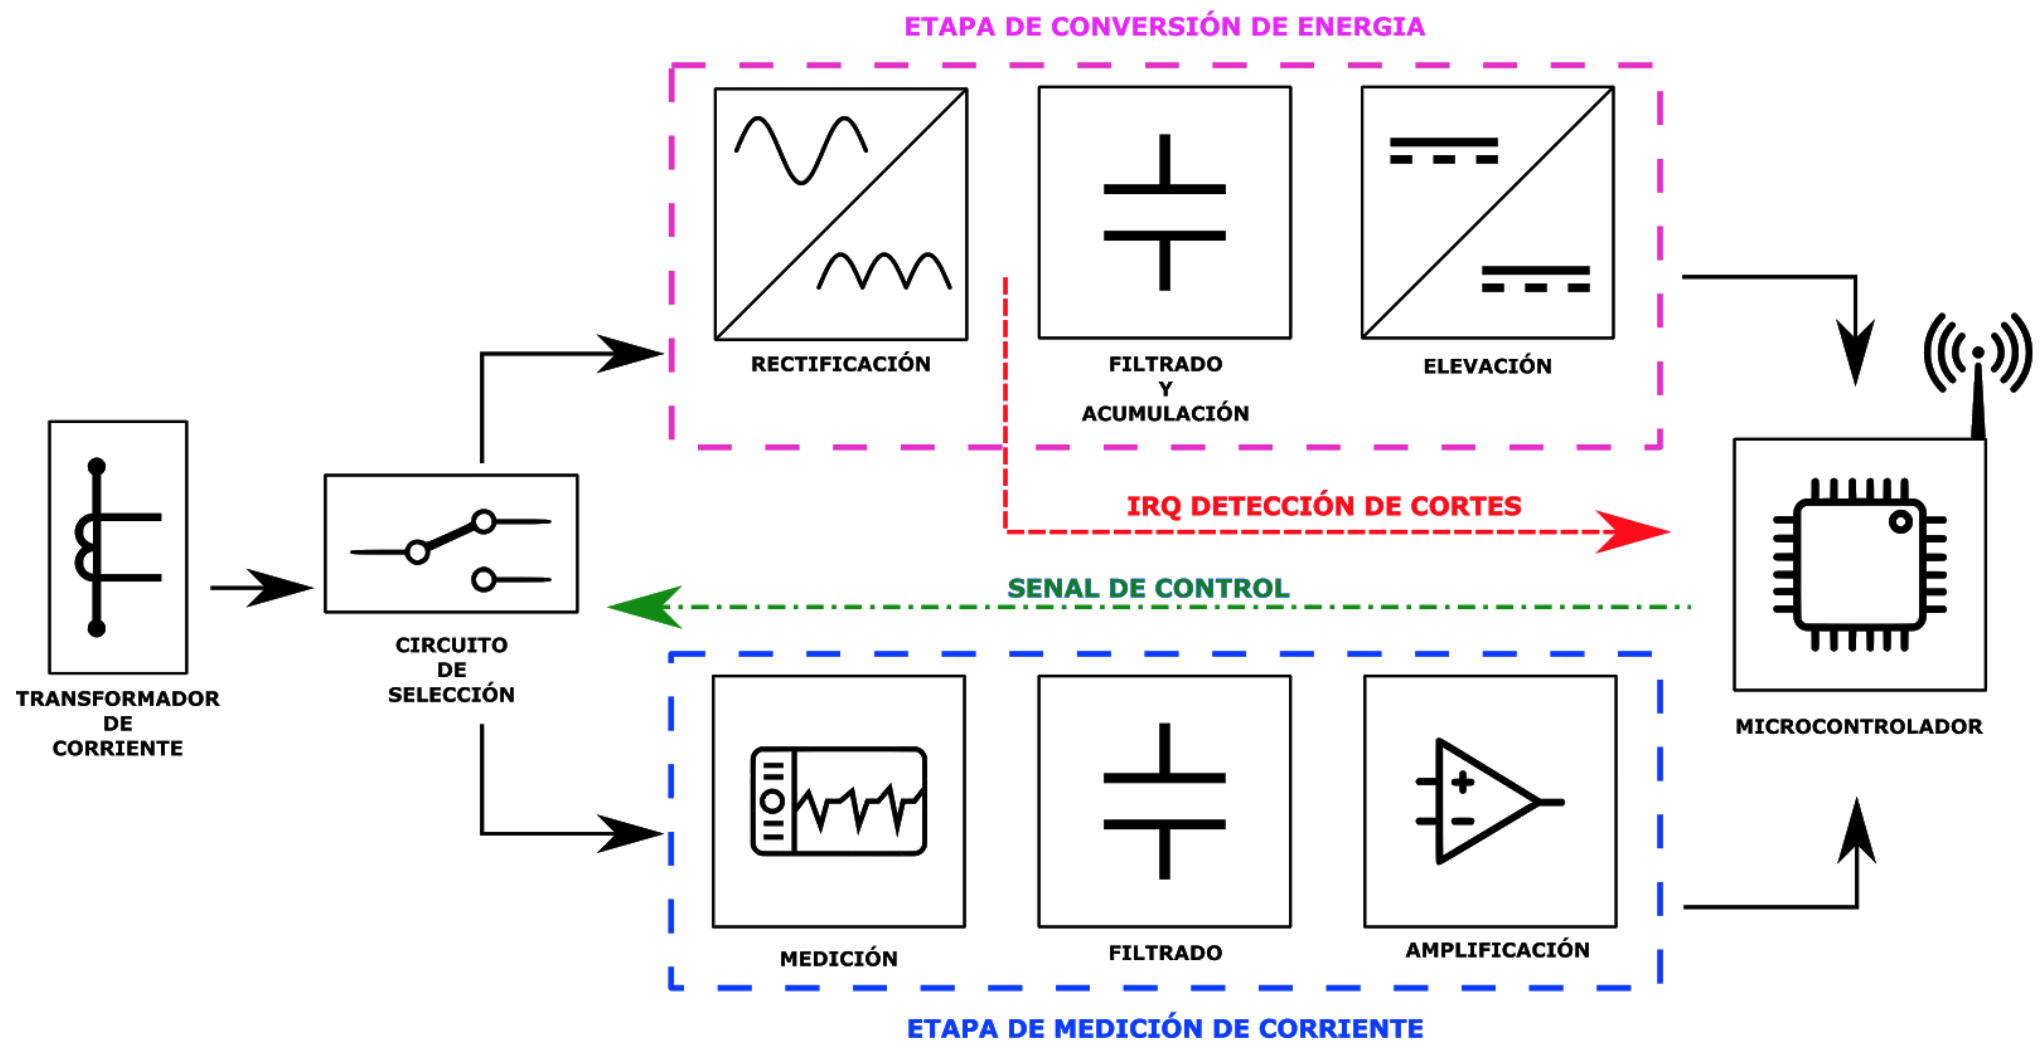
\includegraphics[width=1.0\linewidth]{Figures/diagrama_de_bloques_del_HW}
	\caption{Diagrama de bloques del HW para el nodo a instalar \textit{in situ}.}
	\label{fig:diagramadebloquesdelhw}
\end{figure}
\begin{enumerate}
	\item Circuito de selección de modo: un relay y su circuito de mando controlarán a que etapa del nodo se conectarán los terminales del transformador de corriente.
	\item Etapa de rectificación, acumulación de energía y elevación de tensión: compuesta por rectificador de onda completa, una etapa de filtrado y acumulación, y un circuito elevador de tensión.
	\item Etapa de medición de valor RMS de corriente: un chip dedicado toma la señal de tensión generada en bornes del resistor shunt y calcula el valor RMS. A su salida entrega un valor proporcional de tensión DC.
	\item Microcontrolador: ejecuta la lógica de negocios que rige el comportamiento del nodo, digitaliza mediciones y transmite datos a la red LoRaWAN.
\end{enumerate}
Por otro lado, el sistema también implicó el desarrollo y puesta en funcionamiento de un conjunto de servicios de \textit{backend} (BES) propios del proyecto que cumplen las funciones de:
\begin{itemize}
	\item Recuperación de datos de la red LoRaWAN.
	\item Almacenamiento en una base de datos.
	\item Presentación de los datos al usuario final mediante una interfaz gráfica de usuario.
\end{itemize}
% TODO: \usepackage{graphicx} required

El requisito \ref{requerimiento_LORAWAN} impuso el uso de una red LoRaWAN como protocolo principal para la transmisión de datos generados por los nodos. Para cumplirlo se adoptó la arquitectura presentada en la figura \ref{fig:diagramadebloquesdebes}.\\
% TODO: \usepackage{graphicx} required
\begin{figure}[h!]
	\centering
	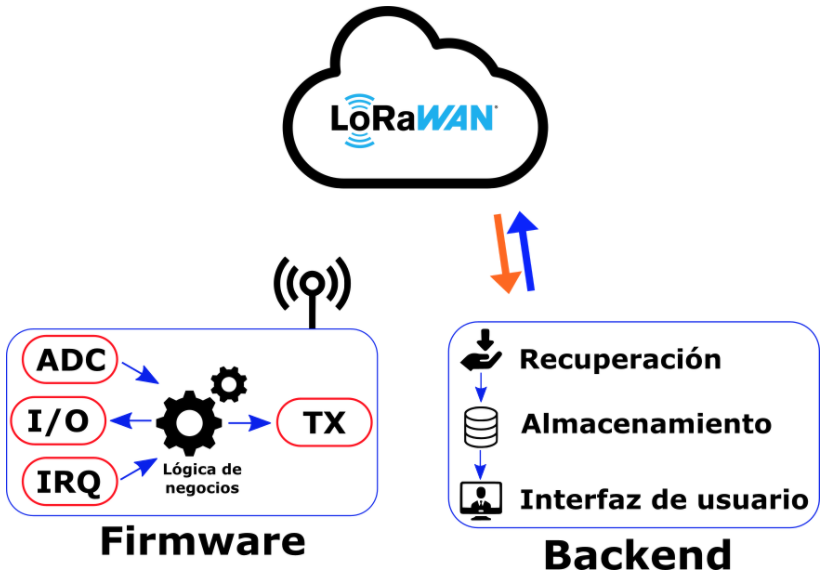
\includegraphics[width=0.8\linewidth]{Figures/diagrama_de_bloques_de_BES}
	\caption{Diagrama de bloques del FW implementado en el MC y su interacción con la red LoRaWAN y los BES privados del sistema.}
	\label{fig:diagramadebloquesdebes}
\end{figure}\\
Las mediciones son tomadas por el HW y transmitidas hacia la red LoRaWAN para luego interactuar con los BES privados que se encargan de recuperar, almacenar y presentar los datos al usuario final.\\

\section{Requerimientos acordados con el cliente}
\label{sec:requerimientos}
\begin{enumerate}
	\item Grupo de requerimientos asociados con hardware:
	\begin{enumerate}
		\item El dispositivo deberá ser de tipo \textit{plug and play}.
		\item El circuito impreso no deberá ocupar un volumen mayor a 10x10x5 cm.
		\item Basarse en un microcontrolador ESP32 y disponer de:
		\begin{enumerate}%[label*=\arabic*.]
			\item 4 entradas analógicas.
			\item 3 salidas digitales.
			\item Unidad UART.
			\item Integrar un módulo de comunicaciones LoRa.
		\end{enumerate}
		\item Deberá tener al menos 12 horas de autonomía de funcionamiento.
		\item Bajo consumo en modo ocioso: el consumo del hardware en total, no deberá superar los 5 mA cuando no está midiendo ni transmitiendo.
		\item El circuito elevador de tensión DC-DC deberá:
		\begin{enumerate}%[label*=\arabic*.]
			\item Funcionar con tensiones menores a 2 V en la entrada.
			\item Otorgar 5 V a la salida.
			\item Ser capaz de otorgar 300 mA a la salida.
		\end{enumerate}
		\item El transformador de corriente (TI) debe:
		\begin{enumerate}%[label*=\arabic*.]
			\item Ser de tipo núcleo partido.
			\item Admitir 100 A de corriente en el circuito primario y un máximo 5 Amperes en el circuito secundario.
		\end{enumerate}
		\item \label{req_relay} El relay encargado de cambiar el modo de operación debe:
		\begin{enumerate}%[label*=\arabic*.]
			\item Ser de tipo doble inversor sin retención.
			\item Su bobina debe poder energizarse con 5 V o menos.
			\item Soportar al menos 5 A de corriente por los contactos.
		\end{enumerate} 
		\item Debe funcionar de manera independiente a la frecuencia de operación de la red 50/60 Hz.
		\item Debe funcionar de manera independiente a la tensión de fase del sistema de distribución 110/220 V.
	\end{enumerate}
	\item Grupo de requerimientos asociados con el firmware:
	\begin{enumerate}
		\item Debe manejar un módulo de comunicación LoRa y protocolo LoRaWAN.
		\item Deberá tener un porcentaje de cobertura de tests unitarios del 60\% como mínimo.
		\item Antes configurarse en modo ocioso, debe desenergizar la etapa de medición de corriente y el módulo de comunicaciones con el objeto de ahorrar energía.
	\end{enumerate}
	
	\item Grupo de requerimientos asociados con los servicios de backend:
	\label{requerimientos_backend}
	\begin{enumerate}
		\item Todos los servicios deben poder correr en una Raspberry Pi 3.
		\item El \textit{software} de los BES se desarrollará en lenguaje Python.
		\item Recuperar los datos de la red LoRaWAN.\label{requerimiento_LORAWAN}
		\item Almacenar los datos en una tabla de MySQL.
		\item Interfaz gr\'{a}fica de usuario basada en Grafana.
	\end{enumerate}
	
	\item Grupo de requerimientos asociados con ensayos de integración y \textit{end-to-end}:
	\begin{enumerate}
		\item El banco de ensayos de hardware debe contar con una carga fantasma de al menos 10 Amperes y permitir realizar interrupciones de corriente de manera programada mediante una computadora adicional tipo Raspberry Pi o de manera manual.
		\item Los BES deben estar operativos al momento de realizar los ensayos.
		\item Se debe contar con un gateway de acceso a una red LoRaWAN como por ejemplo \textit{The Things Network}.
	\end{enumerate}
\end{enumerate}


\section{Detalle del hardware}
\subsection{Transformador de corriente}
Un transformador de corriente o intensidad (TI) es un dispositivo de medición utilizado para producir en su devanado secundario una corriente diferente y proporcional a la que circula por su devanado primario.\\
El principio de operación de un TI no es diferente al de un transformador de potencia convencional. A diferencia de uno de potencia, el devanado primario puede ser de una sola vuelta sobre un núcleo ferromagnético como se ve en la figura \ref{fig:dibujomedicionti}. El devanado secundario suele tener un número mayor de vueltas alrededor del núcleo que depende de que tanto se debe reducir la corriente.\\
Muchos TI tienen una relación estándar de 5 Amperes en el secundario, por ejemplo un TI 200/5 significa que cuando por el primario fluyen 200 amperes en el secundario solo fluyen 5 A. Es decir, el TI tiene una relación de transformación de corriente N de 40 veces.\\
% TODO: \usepackage{graphicx} required
\begin{figure}[h!]
	\centering
	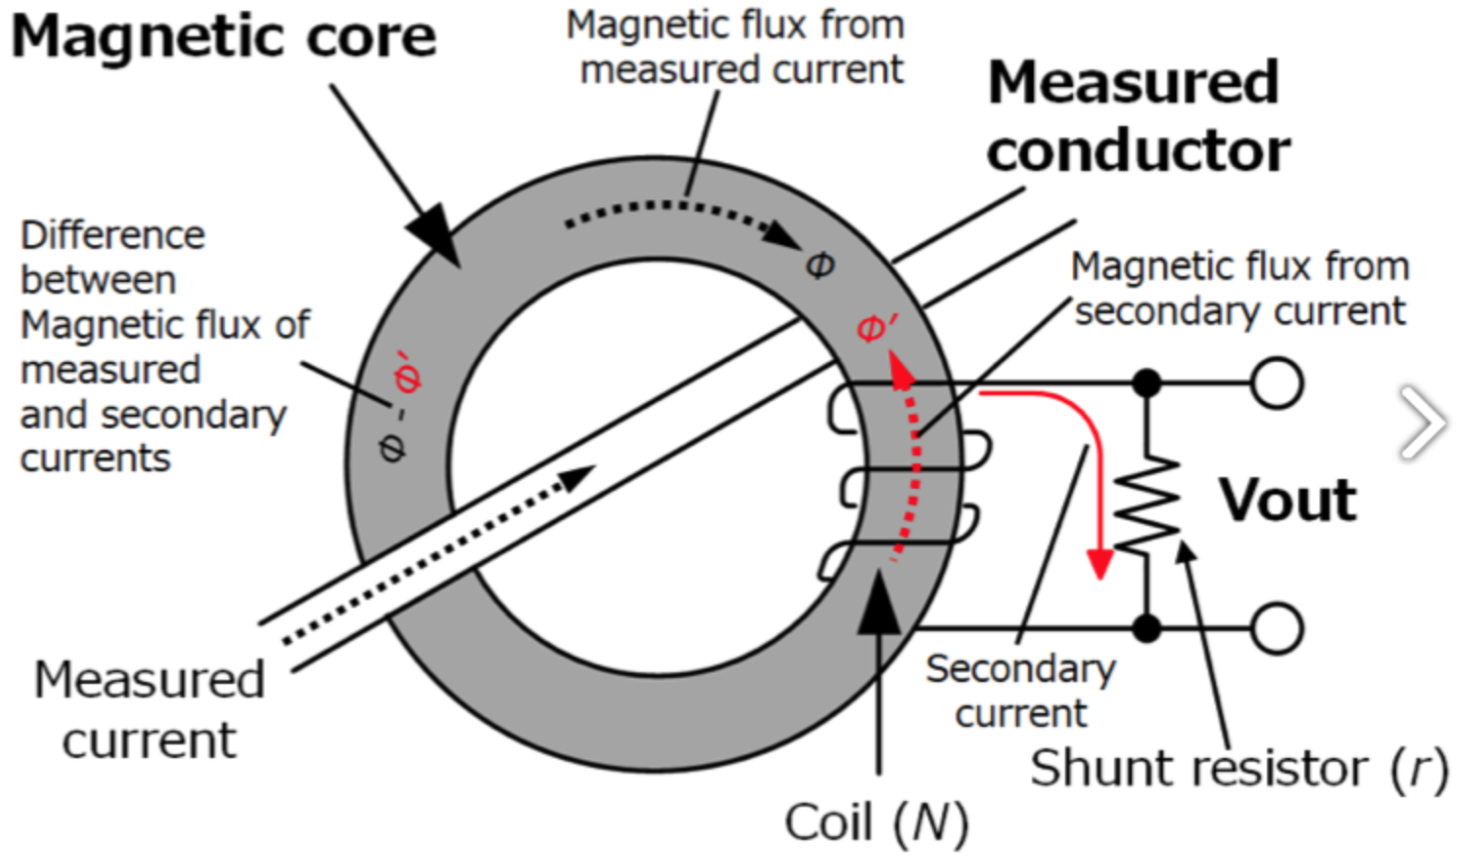
\includegraphics[width=0.8\linewidth]{Figures/dibujo_medicion_TI}
	\caption{Circuito de medición indirecta de corriente mediante un TI \citep{hioki}.}
	\label{fig:dibujomedicionti}
\end{figure}\\
Mediante esta técnica, pequeños instrumentos pueden monitorear grandes valores de corriente manteniendo una distancia segura de las líneas de alta tensión.

\subsection{Circuito de selección}
A partir del lineamiento de que el TI debe estar conectado por defecto a la entrada del rectificador y al resistor shunt cuando se energiza la bobina del relay, el número y la disposición de los contactos resulta un factor relevante al momento de elegir la mejor opción. La variante comercial que cumple con el requisito \ref{req_relay} es la producida por la firma Hongfa modelo HF115F/005-2ZS4A presentada en la figura \ref{fig:relay}.
\begin{figure}[h!]
    \centering
	\begin{subfigure}[b]{0.4\textwidth}
		\centering
		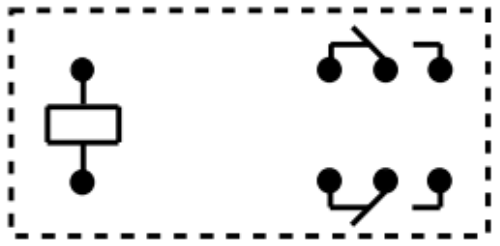
\includegraphics[width=.7\textwidth]{./Figures/relay_pinout}
		\caption{}
		\label{fig:relay_pinout}
	\end{subfigure}
    \centering
	\begin{subfigure}[b]{0.4\textwidth}
		\centering
		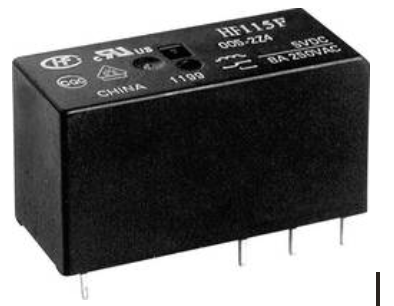
\includegraphics[width=.7\textwidth]{./Figures/relay_encapsulado}
		\caption{}
		\label{fig:relay_encapsulado}
	\end{subfigure}
	\caption{Pinout del relay HF115F/005-2ZS4A (izquierda) y su encapsulado (derecha). Imágenes tomadas de \citep{datasheet_relay}.}
	\label{fig:relay}
\end{figure}

\subsection{Conversión de energía}
Para obtener una tensión continua a partir de una alterna generada por el TI, es necesario implementar un puente rectificador de onda completa.\\
En la actualidad la mayoría de los circuitos rectificadores de onda completa se basan en diodos de silicio de bajo costo. Sin embargo, un diodo de silicio posee una caída de tensión típica de 0,7 V. Esta caída de tensión se traduce en pérdidas por efecto Joule, lo que resulta relevante en dispositivos donde la conversión, acumulación y gestión de energía es crítica. Por lo tanto, se desea maximizar la transferencia de tensión y potencia entre entrada y salida del puente rectificador.\\
Yilmaz \citep{Yilmaz} analiza técnicas de rectificación de onda completa con diferentes tipos de diodos, como así también un arreglo de transistores MOSFET pasivo y activo. Las caídas de tensión simuladas entre la entrada y salida entre un puente rectificador de diodos de silicio y uno pasivo basado en MOSFETs se comparan en la figura \ref{fig:comparacion_diodos_vs_MOSFET}.\\

\begin{figure}[h!]
	\begin{subfigure}{.5\textwidth}
		\centering
		% include first image
		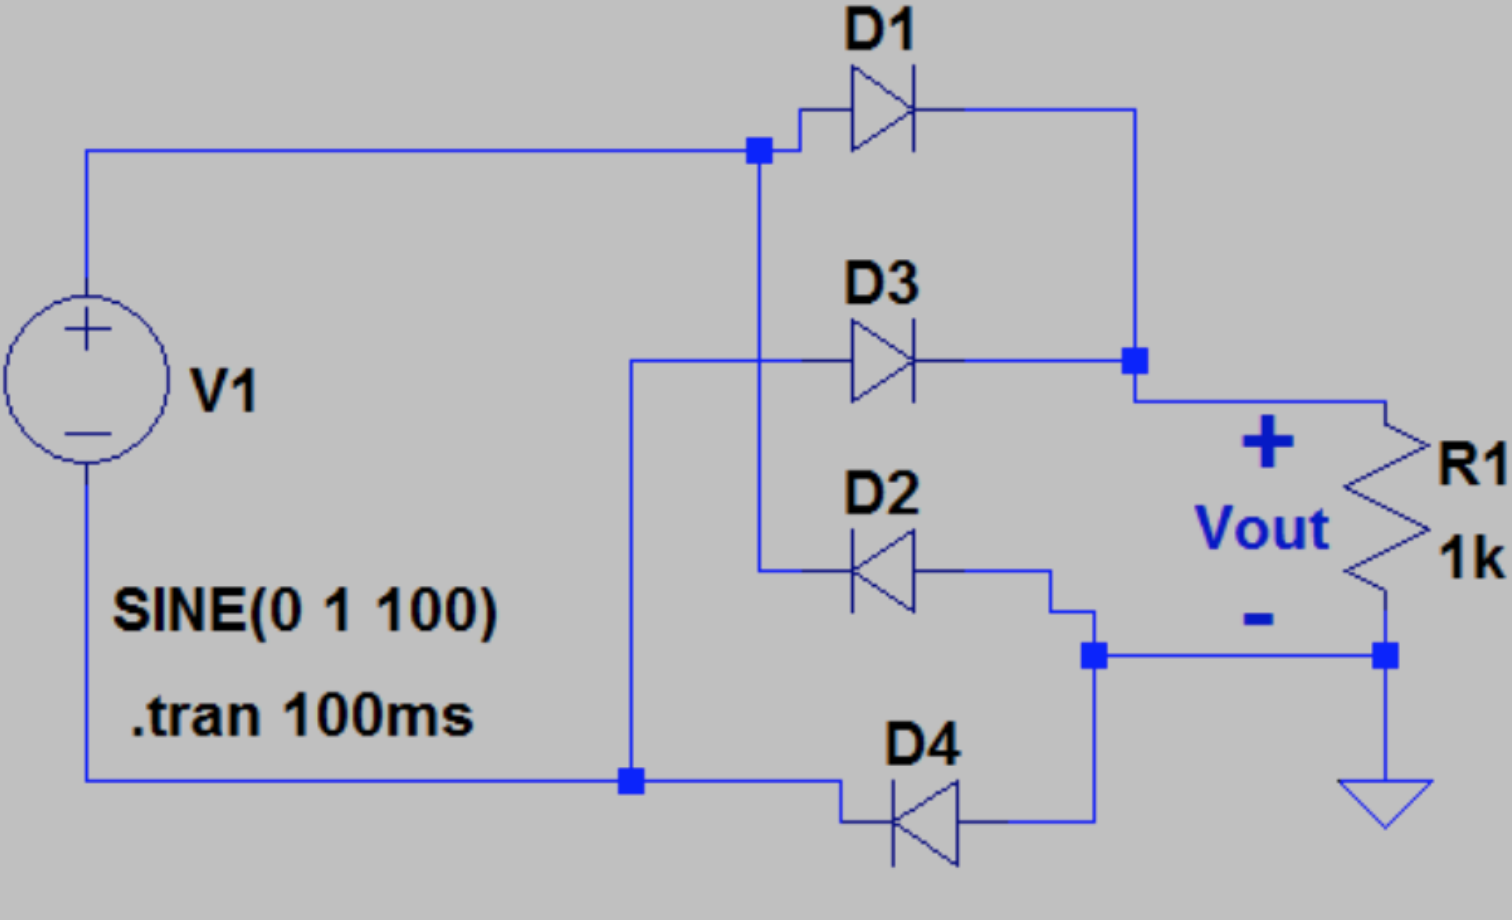
\includegraphics[width=.8\linewidth]{Figures/YILMAZ_silicon_diode_rectifier}  
		\caption{Rectificador basado en diodos de silicio.}
		\label{fig:rect_diodos}
	\end{subfigure}
	\begin{subfigure}{.5\textwidth}
		\centering
		% include second image
		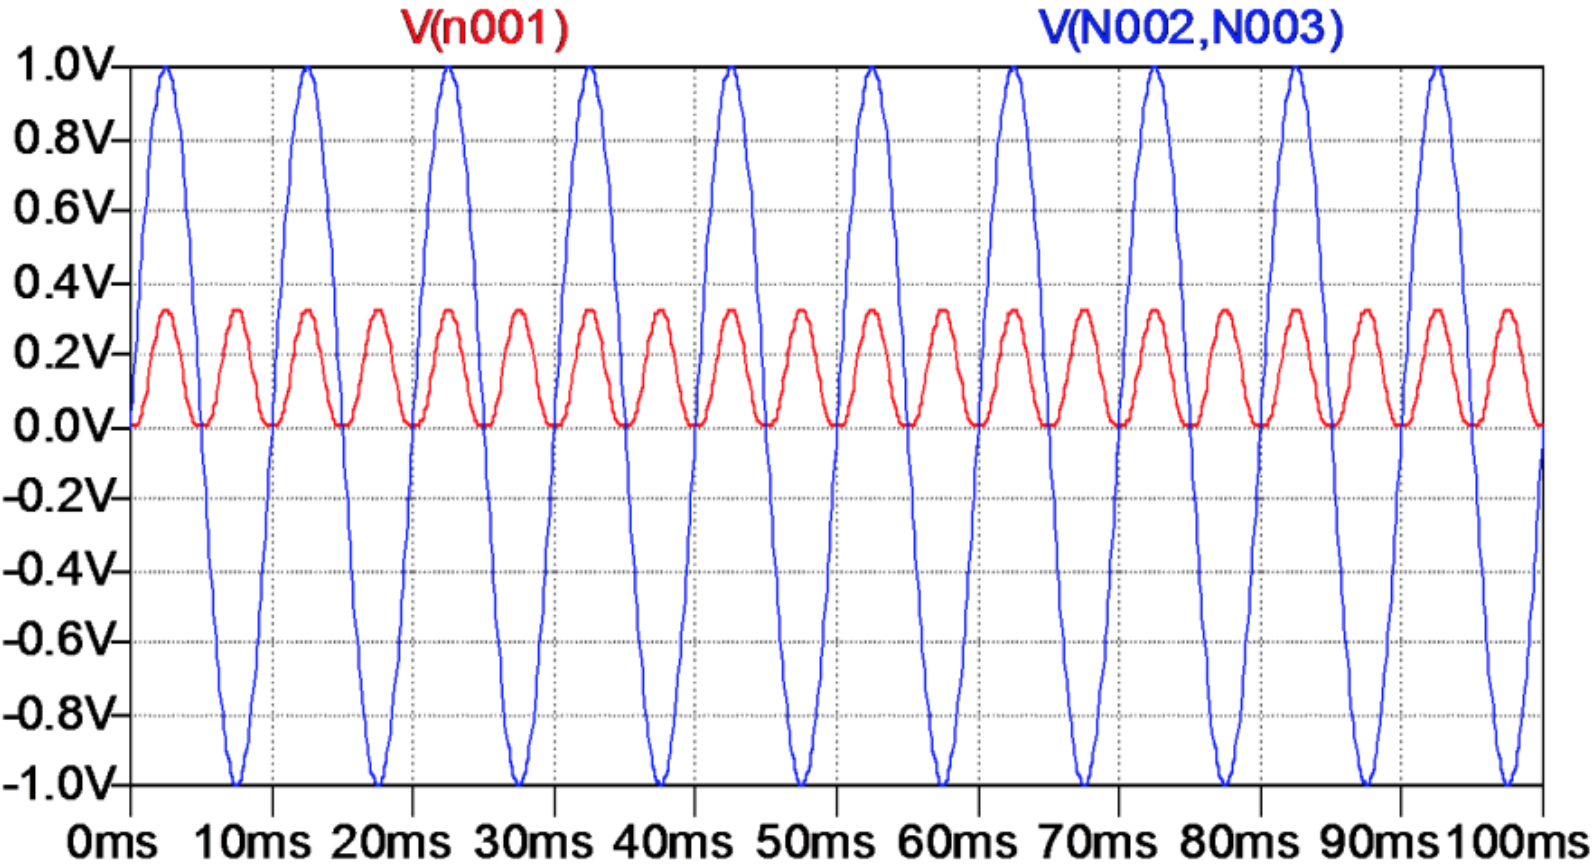
\includegraphics[width=.8\linewidth]{Figures/onda_silicon_rectifier}  
		\caption{Caída de tensión generada por el rectificador de la figura \ref{fig:rect_diodos}.}
		\label{fig:onda_rectificador_diodos}
	\end{subfigure}
	\newline
	\begin{subfigure}{.5\textwidth}
		\centering
		% include third image
		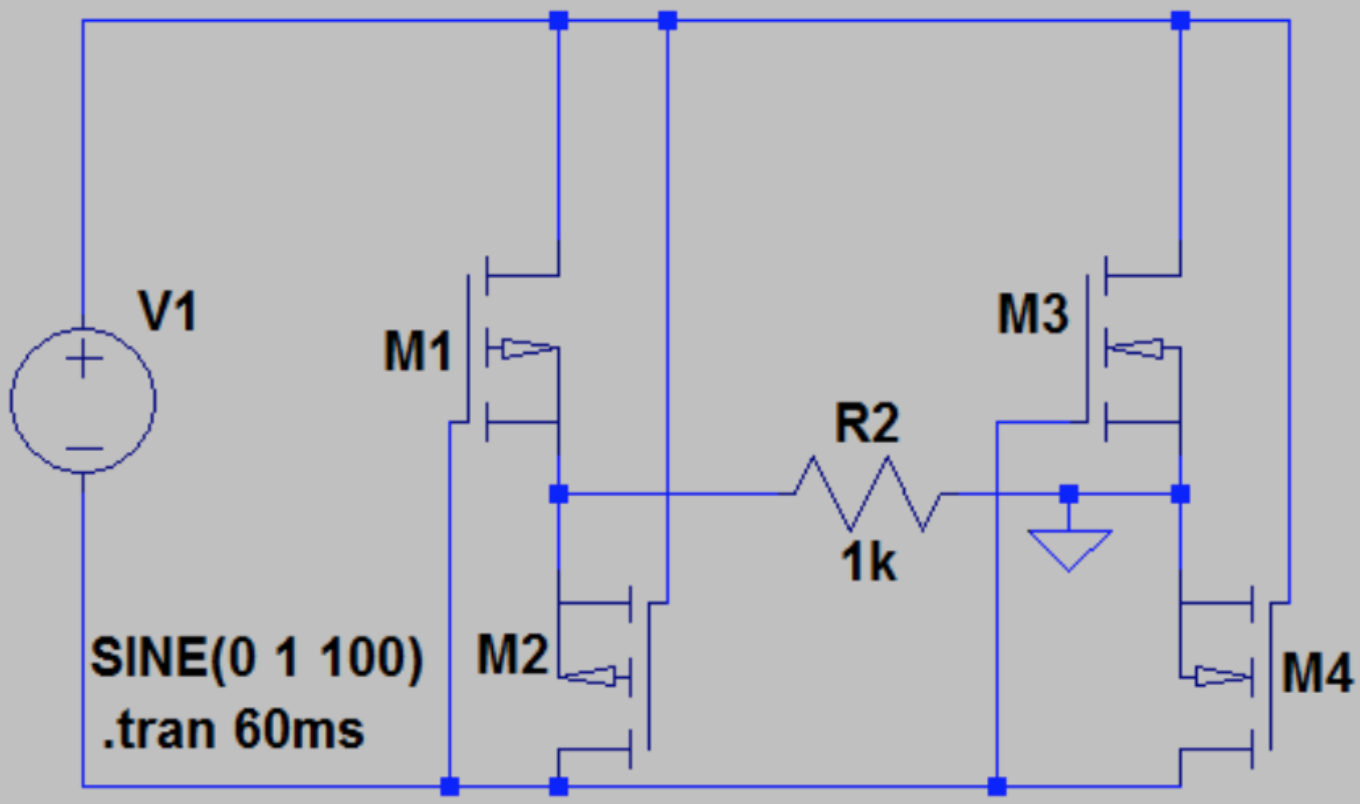
\includegraphics[width=.8\linewidth]{Figures/YILMAZ_passive_MOSFET_rectifier}  
		\caption{Rectificador basado en transistores MOSFET.}
		\label{fig:rect_MOSFET}
	\end{subfigure}
	\begin{subfigure}{.5\textwidth}
		\centering
		% include fourth image
		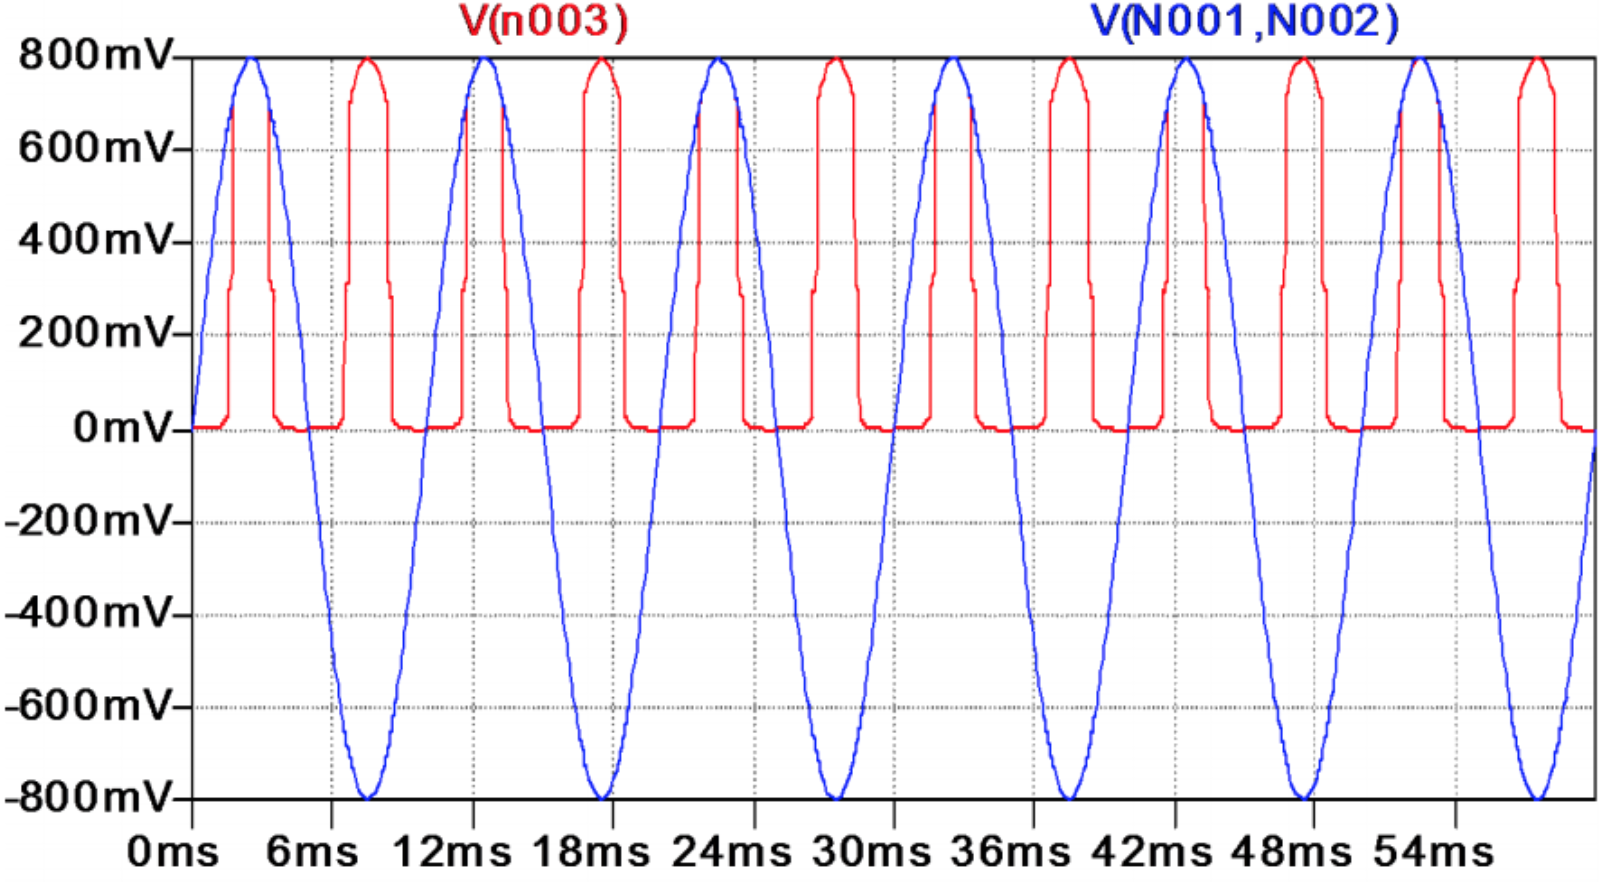
\includegraphics[width=.8\linewidth]{Figures/onda_passive_mosfet_rectifier}  
		\caption{Caída de tensión generada por el rectificador de la figura \ref{fig:rect_MOSFET}.}
		\label{fig:onda_rectificador_MOSFET}
	\end{subfigure}
	\caption{Simulación de rectificadores basados en diodos y MOSFET. Imágenes tomadas de \citep{Yilmaz}.}
	\label{fig:comparacion_diodos_vs_MOSFET}
\end{figure}
Al comparar las simulaciones expuestas en las figuras \ref{fig:onda_rectificador_diodos} y \ref{fig:onda_rectificador_MOSFET} se aprecia que la caída de tensión generada por el rectificador basado en MOSFET al entrar en conducción es menor que uno hecho con diodos y por lo tanto también la potencia disipada en forma de calor.\\

\subsection{Supercapacitor como acumulador de energía}
La decisión de optar por un banco de supercapacitores (SC) como reemplazo total de una batería, se basa principalmente en el entorno donde operará el nodo HW. Las diferencias entre una batería y un SC de interés para este proyecto, son plasmadas en la tabla \ref{tab:batteria_vs_supercap}.\\
Los datos meteorológicos de la provincia de Misiones presentados en \citep{historico_temperaturas}, muestran temperaturas por encima de 30 \textdegree C durante el período de septiembre a marzo. A diferencia de un SC que posee un rango de temperaturas de operación desde los -40 \textdegree C hasta 70 \textdegree C \citep{datasheet_supercap}, condiciones por encima de 35 \textdegree C resultan nocivas para una batería y generan el deterioro prematuro de sus componentes\citep{MA2018653}.\\
%\begin{verbatim}
\begin{table}[h]
	\centering
	\caption{Comparativa entre una batería y un supercapacitor para este proyecto.}
	\begin{tabular}{lcc} 
		\hline
		\multicolumn{1}{c}{}                                                  & Batería         & Supercapacitor                                                                         \\ 
		\hline
		\begin{tabular}[c]{@{}l@{}}Densidad de \\energía (Wh/Kg)\end{tabular} & 265             & 3,9                                                                                    \\
		\begin{tabular}[c]{@{}l@{}}Rango de \\temperatura (\textcelsius)\end{tabular}    & 15 a 35         & -40 a 70                                                                               \\
		Gestión de carga                                                      & V o I constante & \begin{tabular}[c]{@{}c@{}}Determinado por un\\circuito RC serie \citep{ceraolo2014fundamentals}\end{tabular}  \\
		\hline
	\end{tabular}
	\label{tab:batteria_vs_supercap}
\end{table}\\
%\end{verbatim}
Es importante remarcar que la densidad de energía que pueden almacenar también es diferente, una batería tiene una densidad de energía 60 veces mayor que un SC. Sin embargo, para esta aplicación puntual no representó un factor importante a la hora de elegir el acumulador.\\
Por último, el ciclo de carga es más complejo en el caso de una batería. Las etapas de su curva de carga deben ser respetadas según sean a corriente o tensión constante. Esto trae acarreado implementar una electrónica adicional encargada de gestionar estos 2 parámetros. En un capacitor, la curva de carga está definida por un circuito RC serie \citep{ceraolo2014fundamentals}.\\ 

\subsection{Elevación de tensión mediante un conversor DC/DC }
Para proveer al microcontrolador y al resto de la electrónica asociada una tensión DC fija y constante, se optó por emplear un módulo comercial DC/DC ya existente en el mercado que se presenta en la figura \ref{fig:dcdcboost}.\\
% TODO: \usepackage{graphicx} required
\begin{figure}[h!]
	\centering
	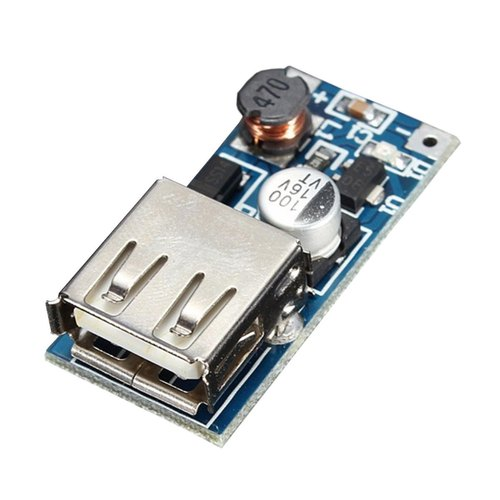
\includegraphics[width=0.4\linewidth]{Figures/dcdc_boost}
	\caption{Módulo comercial DC/DC en topología boost utilizado para alimentar la electrónica.}
	\label{fig:dcdcboost}
\end{figure}\\
Su topología interna es \textit{boost} o elevador de tensión. En el HW del sistema, cumple la función de llevar la tensión variable del SC conectado a su entrada a una fija de 5 V. 
A su entrada admite tensiones variables desde 0,9 V hasta 5 V y puede otorgar hasta 500 miliamperes de corriente a la salida.

\subsection{Microcontrolador y firmware}
El MC es el ente encargado de ejecutar la lógica de negocios acorde a la tarea que debe cumplir el HW. En el mercado existe una amplia gama de fabricantes de placas de desarrollo que permiten acelerar la etapa de prototipado y validación de diseño.\\
La placa de desarrollo elegida para el prototipo fue la LoPy 4 producida por la firma Pycom que se presenta en la figura \ref{fig:lopy4} . En su interior alberga un ESP32, 8 Megabytes de memoria flash, transceptores de radio LoRa y 802.11 y un regulador de tensión.\\
\begin{figure}[h]
	\centering
	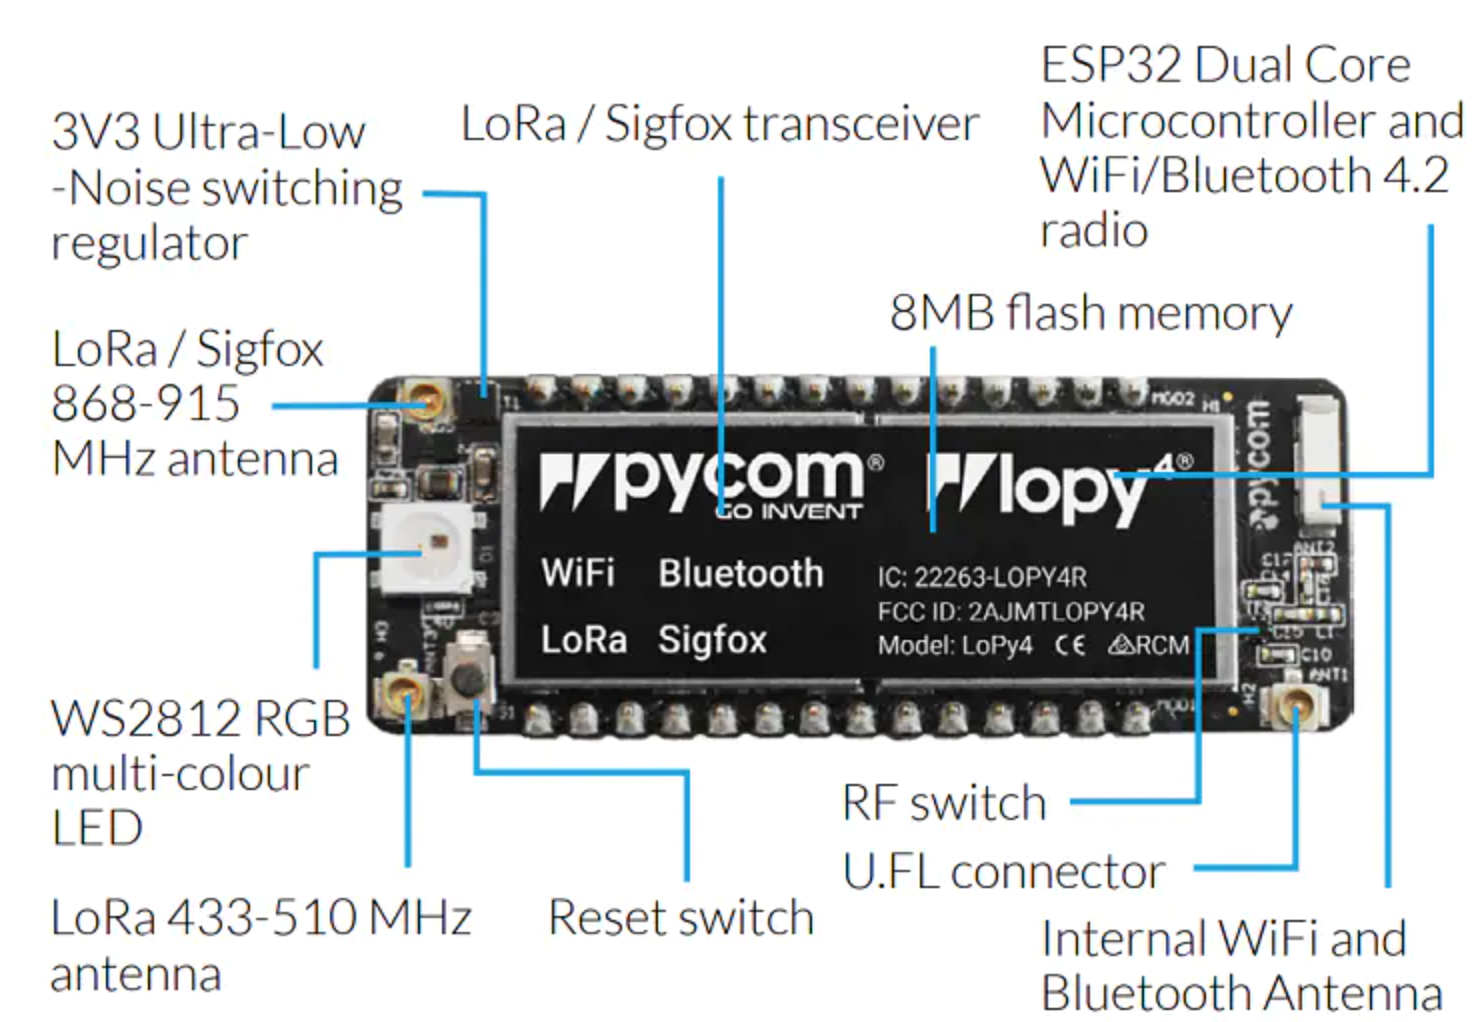
\includegraphics[width=0.95\linewidth]{Figures/lopy4}
	\caption{Placa de desarrollo LoPy 4 \citep{lopy4}.}
	\label{fig:lopy4}
\end{figure}\\
El lenguaje de programación de la LoPy4 es Micropython \citep{micropy}, un lenguaje de alto nivel lanzado por primera vez en el año 2014. Desde su lanzamiento y hasta la fecha de desarrollo de este trabajo, se presenta como una variante de Python atractiva para prototipar FW sobre microcontroladores utilizando el paradigma de programación orientada a objetos.\\


\section{Detalle del software}
\subsection{Red LoRaWAN}
LoRaWAN (Long Range Wide Area Network) es un protocolo de control de acceso al medio (MAC - \textit{Medium Acces Control}) definido por \textit{LoRa Aliance} \citep{lora_alliance}. Tiene por objeto permitir la conexión de nodos de baja potencia, generalmente alimentados a batería y sin capacidad de manejo de protocolos de enrutamiento, con aplicaciones finales conectadas a Internet mediante una conexión inalámbrica de largo alcance utilizando modulación LoRa.\\
Las puertas de enlace (GW - \textit{gateways}), están conectadas al servidor central mediante conexiones IP (Internet Protocol) estándar, cumpliendo la función de puente, es decir, convierten los paquetes de radiofrecuencia (RF) en paquetes IP y viceversa \ref{fig:arqlorawan}.\\
% TODO: \usepackage{graphicx} required
\begin{figure}[h]
	\centering
	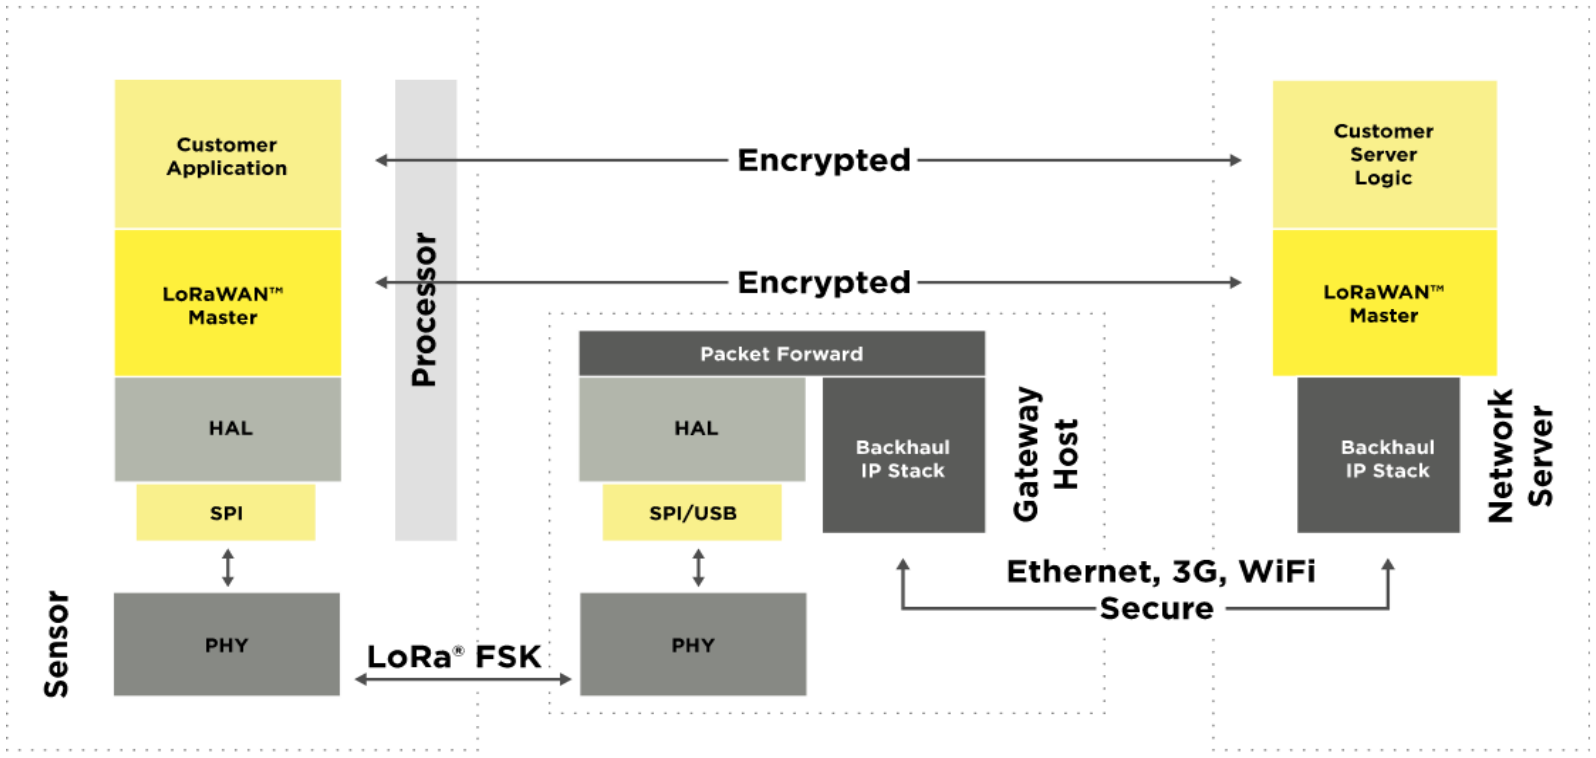
\includegraphics[width=1.05\linewidth]{Figures/arq_lorawan_2}
	\caption{Arquitectura de una red LoRaWAN y sus posibles integraciones con terceras partes \citep{lora_alliance}.}
	\label{fig:arqlorawan}
\end{figure}\\
El protocolo LoRaWAN no es un protocolo IP, por lo tanto, los paquetes del mismo necesitan de un enrutamiento y procesamiento correspondiente antes de ser entregados a la aplicación final.\\
La figura \ref{fig:sensor-gw-architecture-lora} presenta la topología tipo ``estrella de estrellas`` que adopta una red LoRaWAN. En ella, los \textit{gateways} retransmiten los mensajes recibidos de los nodos finales hacia un servidor central. La comunicación inalámbrica entre nodos y gateways aprovecha las características propias de la capa física, lo que permite establecer enlaces desde un nodo hacia uno o más de estos gateways.\\
% TODO: \usepackage{graphicx} required
\begin{figure}[h]
	\centering
	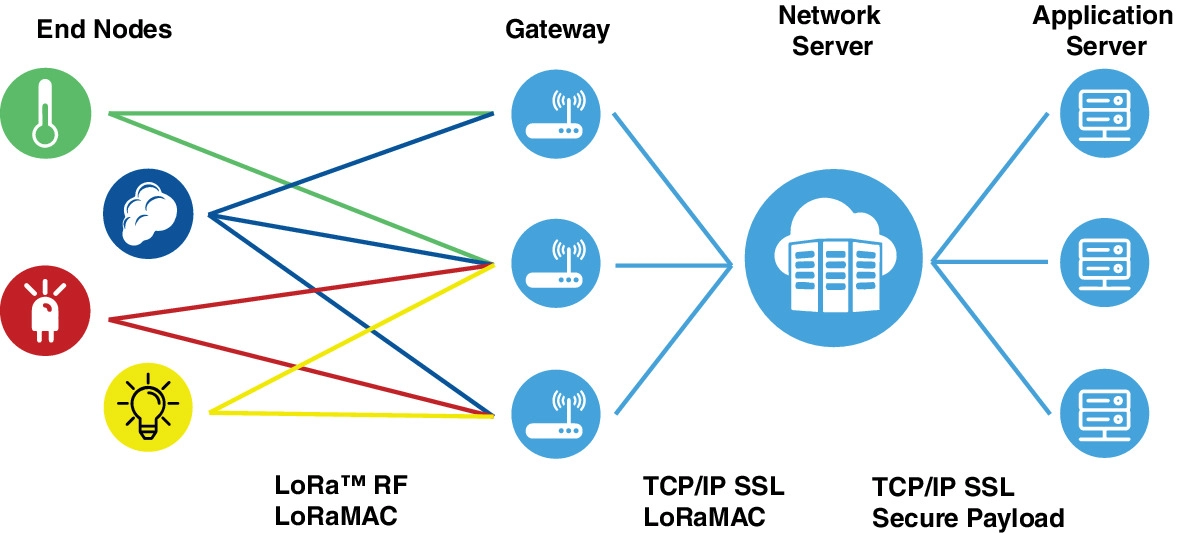
\includegraphics[width=0.9\linewidth]{Figures/sensor-gw-architecture-lora}
	\caption{Topología de una red LoRaWAN y la interacción entre los diferentes miembros \citep{lora_alliance}.}
	\label{fig:sensor-gw-architecture-lora}
\end{figure}

\subsection{Motor de base de datos}
Una base de datos almacena la información de manera ordenada en tablas o estructuras de datos. Las distintas aplicaciones pueden ejecutar consultas para solicitar la parte de esos datos que necesiten en ese momento.\\
Las bases de datos más utilizadas para aplicaciones \textit{web} son las basadas en un modelo relacional, también conocidas como bases de datos SQL (Structured Query Language). Sin embargo, en años recientes se han popularizado las llamadas bases de datos no relacionales o NoSQL. Estas últimas están orientadas a documentos y almacenan información de un mismo tipo en la forma de clave-valor.\\
Por su naturaleza, este proyecto parece indicado para utilizar una base de datos no relacional. Ya que solo almacena registros de un tipo y no necesita crear relaciones complejas entre distintas tablas de datos.\\
En principio se pensó en utilizar \textit{Elasticsearch} \citep{elasticsearch}, un servidor de búsqueda de texto basado en documentos JSON. Se trata de una herramienta open source que se integra con Grafana, la herramienta para el desarrollo de la interfaz gráfica \citep{grafana}.\\
Sin embargo, en las primeras pruebas llevadas a cabo se pudo apreciar que el consumo de memoria y procesamiento eran muy elevados si se lo implementaba en un hardware de bajas prestaciones como las \textit{Raspberry Pi} \citep{raspi}. Finalmente, se optó por utilizar MariaDB \citep{mariadb}, una base de datos del tipo SQL, también open source, con menos demanda de recursos y muy popular en aplicaciones \textit{web}.\\

\subsection{Interfaz gráfica de usuario}
Una vez recuperados los datos de la red LoRaWAN y almacenados en la base de datos, la interfaz de usuario del sistema presenta al usuario final del centro de operaciones los datos recolectados por cada nodo.\\
Una interfaz gráfica como la que se visualiza en la figura \ref{fig:guirequeridaporelcliente}, se encarga de presentar al usuario final los últimos datos adquiridos por cada nodo. De esta manera, se puede identificar de manera simple mediante un punto verde o rojo sobre el mapa si la línea monitoreada presenta un problema.
% TODO: \usepackage{graphicx} required
\begin{figure}[h!]
	\centering
	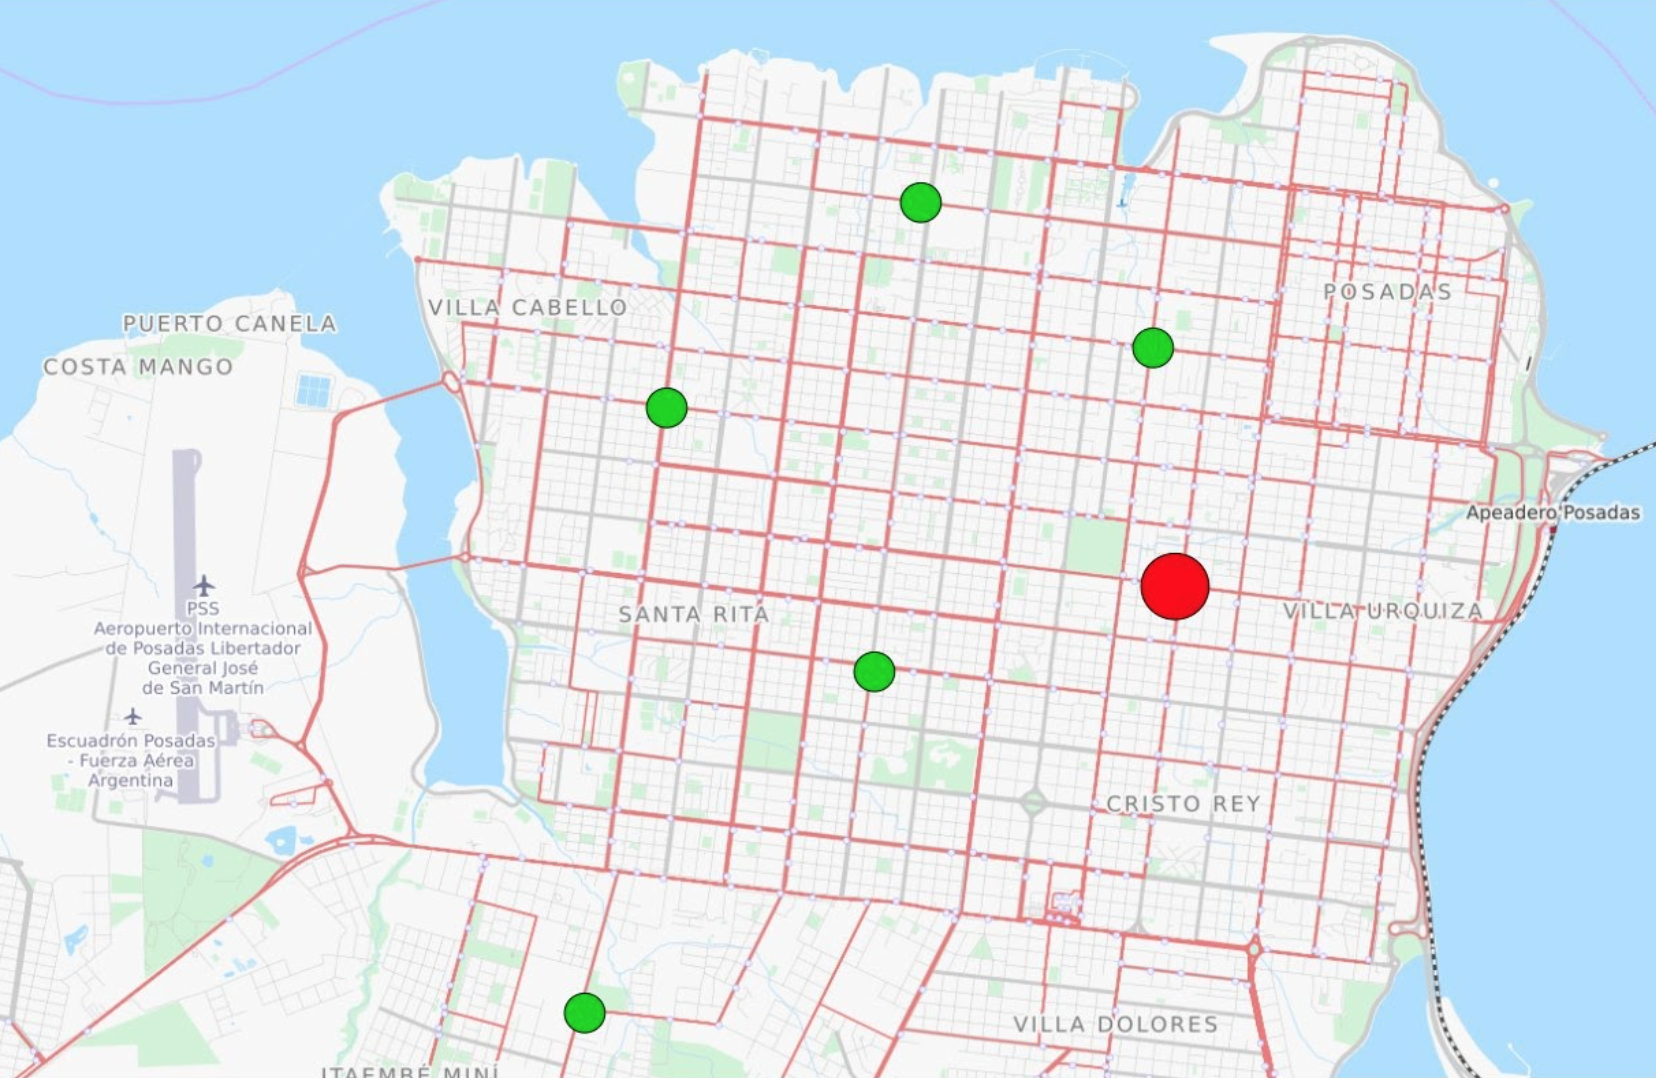
\includegraphics[width=0.9\linewidth]{Figures/GUI_requerida_por_el_cliente}
	\caption{Interfaz gráfica que muestra los datos capturados de cada nodo del sistema.}
	\label{fig:guirequeridaporelcliente}
\end{figure}\\
Para la presentación de la información se optó por Grafana, una aplicación \textit{web} de código abierto para el análisis y visualización de datos \citep{grafana}.\\
Para mejorar aun más la experiencia del usuario se complementa con el plug-in \textit{Worldmap Panel}, que permite mostrar información temporal sobre un mapa. Esta información se presenta como círculos en las coordenadas donde se encuentra ubicado el nodo que genera la información.\\
